% ============================================================
% B-layout.tex  (2026-11-17)
% The two-ancilla layout (search name: layout B) of the [[5,1,2]]_3 code: 5 data qutrits and two ancillas N and E
% on a square lattice with 8 nearest-neighbour couplers.
%   q4(0,2) N(1,2); q1(0,1) q2(1,1) E(2,1); q0(0,0) q3(1,0)   (x right, y up)
% Couplers: q0-q1, q0-q3, q1-q2, q2-q3, q1-q4, N-q4, N-q2, E-q2; no diagonals.
% Roles (BRIEF-layoutB.md, encoders/layoutB_verify.out):
%   check rounds: q0-q1 (4 gates), q1-q2 (4), q1-q4 (4), q2-q3 (4), N-q2 (3),
%                 N-q4 (2), E-q2 (3); 24 in all
%   logical gates (SWAP_{2,3} in H-bar, CZ_{2,3} in S-bar): q2-q3 only
%   encoder (H on q2,q3,q4; CNOT 3->0, CNOT 4->1, CNOT_INV 2->1, CNOT 1->0):
%                 q0-q1, q0-q3, q1-q2, q1-q4; q0-q3 is encoder only (dashed)
% N reads G2 (Z type), then G4 (X type); E reads G1 (Z), then G3 (X).
% Palette and sizes as a1-layout.tex. Drawn at final printed size (scale 1).
% ============================================================
\documentclass[tikz,border=1pt]{standalone}
\usepackage{amsmath,amssymb}
\usetikzlibrary{calc}

% ---------- palette: exactly the paper's; no other hues ----------
\definecolor{Zcol}{HTML}{FF1744}
\definecolor{Xcol}{HTML}{00B7FF}
\definecolor{SwapCol}{HTML}{8E44AD}
\colorlet{Xtint}{Xcol!26}
\colorlet{Ztint}{Zcol!17}
\colorlet{XRim}{Xcol}
\colorlet{ZRim}{Zcol}
\colorlet{XText}{Xcol!80!black}
\colorlet{ZText}{Zcol!85!black}
\colorlet{GateCol}{SwapCol}       % q2-q3 coupler of the logical gates
\colorlet{EncCol}{black!75}       % encoder-only couplers
\colorlet{CountCol}{black!60}     % gate counts per coupler

% ---------- sizes (as ancilla-layouts.tex) ----------
\def\u{1.40}          % lattice step (cm)
\def\rq{0.17}         % data circle radius (cm), the paper's \qdR = 4.8pt
\def\ss{0.40}         % ancilla square side (cm)
\def\lab{0.37}        % readout label distance from the ancilla centre (cm)
\def\cnt{0.11}        % gate-count label offset from its coupler (cm)

\tikzset{
  every node/.style={font=\footnotesize},
  data/.style={circle,inner sep=0pt,minimum size=2*\rq cm,line width=0.7pt,
               draw=black,fill=white,font=\scriptsize},
  check/.style={line width=0.9pt,draw=black},
  gate/.style={line width=1.2pt,draw=GateCol,line cap=round},
  enc/.style={line width=0.9pt,draw=EncCol,dash pattern=on 2.4pt off 1.8pt,line cap=butt},
  encedge/.style={enc,dash phase=0.82pt},   % lattice edges: equal stubs at both ends
  count/.style={font=\scriptsize,text=CountCol,inner sep=0pt},
  readout/.style={font=\footnotesize,inner sep=0pt},
}

% ancilla that reads a Z-type and then an X-type stabilizer: rounded square
% split along its diagonal, Z tint and rim lower left, X tint and rim upper right
% #1 position, #2 label
\newcommand{\DualSite}[2]{%
  \begin{scope}[shift={(#1)}]
    \def\h{0.5*\ss}
    \pgfmathsetmacro{\cl}{0.5*\ss+0.04}  % clip triangles just cover the rim (tight bounding box)
    \def\sq{(-\h,-\h) rectangle (\h,\h)}
    \begin{scope}
      \clip (-\cl,\cl) -- (-\cl,-\cl) -- (\cl,-\cl) -- cycle;
      \fill[Ztint,rounded corners=1.2pt] \sq;
      \draw[ZRim,line width=0.7pt,rounded corners=1.2pt] \sq;
    \end{scope}
    \begin{scope}
      \clip (-\cl,\cl) -- (\cl,\cl) -- (\cl,-\cl) -- cycle;
      \fill[Xtint,rounded corners=1.2pt] \sq;
      \draw[XRim,line width=0.7pt,rounded corners=1.2pt] \sq;
    \end{scope}
    \node[font=\footnotesize,inner sep=0pt] at (0,0) {#2};
  \end{scope}}
% readout label next to an ancilla: #1 ancilla, #2 direction (angle), #3 text
\newcommand{\Readout}[3]{\node[readout,anchor=#2+180] at ($(#1)+(#2:\lab)$) {#3};}
\newcommand{\NReads}{$\textcolor{ZText}{G_2},\,\textcolor{XText}{G_4}$}
\newcommand{\EReads}{$\textcolor{ZText}{G_1},\,\textcolor{XText}{G_3}$}
% key glyphs, centred 0.5ex above the baseline
\newcommand{\KeyLine}[1]{\tikz[baseline=-0.5ex]\draw[#1] (0,0) -- (0.55,0);}
\newcommand{\KeyDual}{\tikz[baseline=-0.5ex]{\def\ss{0.30}\DualSite{0,0}{}}}

\begin{document}
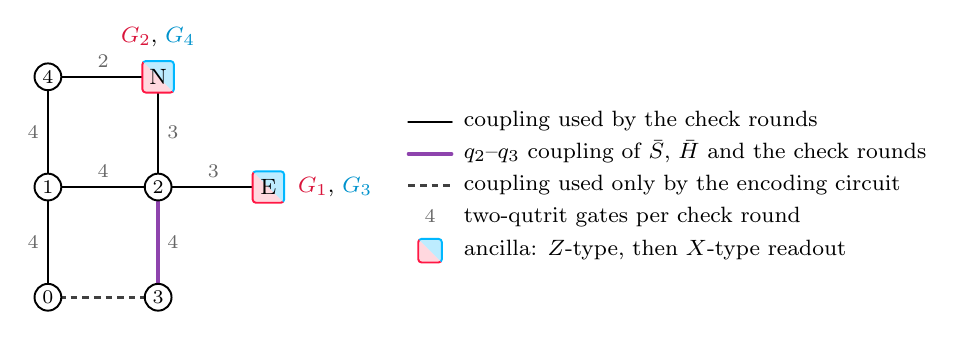
\begin{tikzpicture}[line cap=round,line join=round]

% ---------- two-ancilla layout lattice, q2 at the origin ----------
\coordinate (q4) at (-\u, \u); \coordinate (N)  at (0, \u);
\coordinate (q1) at (-\u,0);   \coordinate (q2) at (0,0);   \coordinate (E)  at (\u,0);
\coordinate (q0) at (-\u,-\u); \coordinate (q3) at (0,-\u);

% couplers: encoder only (dashed), check rounds (black), logical gates (purple)
\draw[encedge,shorten <=\rq cm,shorten >=\rq cm] (q0) -- (q3);
\foreach \a/\b in {q0/q1,q1/q2,q1/q4,q4/N,q2/N,q2/E} \draw[check] (\a) -- (\b);
\draw[gate,shorten <=\rq cm+0.5pt,shorten >=\rq cm+0.5pt] (q2) -- (q3);

% two-qutrit gates per check round on each coupler (encoders/layoutB_verify.out)
\node[count,anchor=east]  at ($(q0)!0.5!(q1)+(-\cnt,0)$) {4};
\node[count,anchor=east]  at ($(q1)!0.5!(q4)+(-\cnt,0)$) {4};
\node[count,anchor=south] at ($(q1)!0.5!(q2)+(0,\cnt)$)  {4};
\node[count,anchor=west]  at ($(q2)!0.5!(q3)+(\cnt,0)$)  {4};
\node[count,anchor=south] at ($(q4)!0.5!(N)+(0,\cnt)$)   {2};
\node[count,anchor=west]  at ($(q2)!0.5!(N)+(\cnt,0)$)   {3};
\node[count,anchor=south] at ($(q2)!0.5!(E)+(0,\cnt)$)   {3};

% qutrits
\DualSite{N}{N}
\DualSite{E}{E}
\foreach \i in {0,...,4} \node[data] at (q\i) {\i};
\Readout{N}{90}{\NReads}
\Readout{E}{0}{\EReads}

% ---------- key (right of the lattice) ----------
\node[anchor=west,inner sep=0pt,align=left,font=\footnotesize] at (\u+1.75,0) {%   % clear of E's readout label
  \begin{tabular}{@{}c@{\hspace{0.45em}}l@{}}
    \KeyLine{check} & coupling used by the check rounds\\[2pt]
    \KeyLine{gate}  & $q_2$--$q_3$ coupling of $\bar S$, $\bar H$ and the check rounds\\[2pt]
    \KeyLine{enc}   & coupling used only by the encoding circuit\\[2pt]
    \textcolor{CountCol}{\scriptsize 4} & two-qutrit gates per check round\\[2pt]
    \KeyDual        & ancilla: $Z$-type, then $X$-type readout
  \end{tabular}};

\end{tikzpicture}
\end{document}
